\section{Results and Discussion}

Evolutionary innovations are adaptive traits that allow a lineage to cross a functional barrier and gain access to new niches. \cite{mayr1963animal} They are often framed as ``key innovations'' that can promote rapid diversification in the groups that evolve them \cite{heard1995key, hunter_key_1998}, and the search for key innovations has become a major component of modern macroevolutionary studies. \cite{maia_key_2013, rabosky_diversity-dependence_2013} However, despite the obvious importance of evolutionary innovations in the history of life on Earth, innovative traits rarely show a direct link with increased diversification. \cite{cracraft_origin_1990, vermeij_innovation_2001, vermeij_ecology_2007, vermeij_crucibles_2012, alfaro_does_2009, givnish_molecular_2000, hodges_spurring_1995, schluter2000ecology, brawand_genomic_2014, mitter_phylogenetic_1988}

Evolutionary innovations are also traditionally thought to reduce extinction rates, \cite{heard1995key} but this may not be the case if innovation facilitates the evolution of specialist phenotypes sensitive to ecological disturbance. \cite{futuyma_evolution_1988, givnish_adaptive_1998} Innovation may also exhibit niche-specific effects on extinction rates if the innovative trait involves a performance trade-off. \cite{schluter2000ecology} Specifically, performance may increase in new niches at the cost of competitive exclusion and eventual extirpation from previously accessible niches.

We examined the potential cost of evolutionary innovation by using a classic example: pharyngognathy. \cite{liem_evolutionary_1973} Pharyngognathy involves multiple modifications of the jaw apparatus in the back of the throat that allow a fish to generate high bite force, which likely enables pharyngognathous fishes to exploit hard-shelled and processing-intensive prey items. \cite{wainwright_biomechanical_1987} However, these modifications reduce pharyngeal gape, which may alter the maximum size of prey that can be easily swallowed. \cite{wainwright_evolution_2012}

Several lineages within the spiny-finned fishes have independently evolved pharyngognathy, including wrasses, surfperches, damselfish, marine halfbeaks, flyingfishes, and cichlids. \cite{wainwright_evolution_2012} Most of these lineages live in shallow marine habitats, except for cichlids, which occur mostly in tropical freshwaters. Cichlids are especially well known for their tendency to undergo rapid speciation and accumulate exceptionally large species richness in spatially confined assemblages, particularly in Lakes Victoria, Malawi, and Tanganyika in eastern Africa. \cite{greenwood1981haplochromine, seehausen_african_2006}

Each of these lineages has interacted with non-pharyngognathous spiny-finned lineages in different ways. In marine habitats, pharyngognathous lineages such as wrasses, parrotfishes and damselfishes have existed alongside closely related nonpharyngognathous spiny-finned fishes for tens of millions of years. \cite{wainwright_evolution_2012} In Lakes Victoria and Malawi, cichlids initially radiated in the complete absence of any nonpharyngognathous spiny-finned fish lineages. Unfortunately, in the 1950s, a nonpharyngognathous predatory fish, the Nile perch, Lates niloticus, was introduced into Lake Victoria, facilitating a cichlid mass extinction. \cite{witte_destruction_1992} In Lake Tanganyika, which hosts an older cichlid radiation than Victoria and Malawi, non-pharyngognathous Lates species and the pharyngognathous cichlids coexist, albeit with many fewer cichlid species and a lower speciation rate than the other two radiations. \cite{seehausen_african_2006, tiercelin1991lake}

Comparative dietary data reveal that pharyngognathy has ecological consequences for the marine lineages that possess the trait. Unlike cichlids, which can sometimes evolve into predatory niches free from competition with predators like Nile perch, marine pharyngognaths always occur alongside typical nonpharyngognathous fish-eating lineages. \cite{wainwright_evolution_2012} We surveyed diet data across a phylogeny of marine spiny-finned fishes, including four marine transitions to pharyngognathy as well as other spiny-finned species occurring in the same environments as those four lineages, and measured rates of dietary evolution for fish and processing-intensive prey like plants and hard-shelled animals. We analyzed diet both as a continuous character using Brownian motion and as a categorical variable using stochastic character mapping (see Methods). In both cases, we examined whether fishes with pharyngognathy had different rates of dietary evolution or rates of transition to a specialist diet for fish prey and processing-intensive prey. Pharyngognathous marine fishes evolved into niches favoring processing-intensive prey items at a much higher rate than other spiny-finned fishes (Figure \ref{FJ_fig1}). However, pharyngognaths evolved into fish-eating niches more slowly, suggesting that the evolution of the innovation may compromise access to this niche.

\begin{figure}
    \centering
    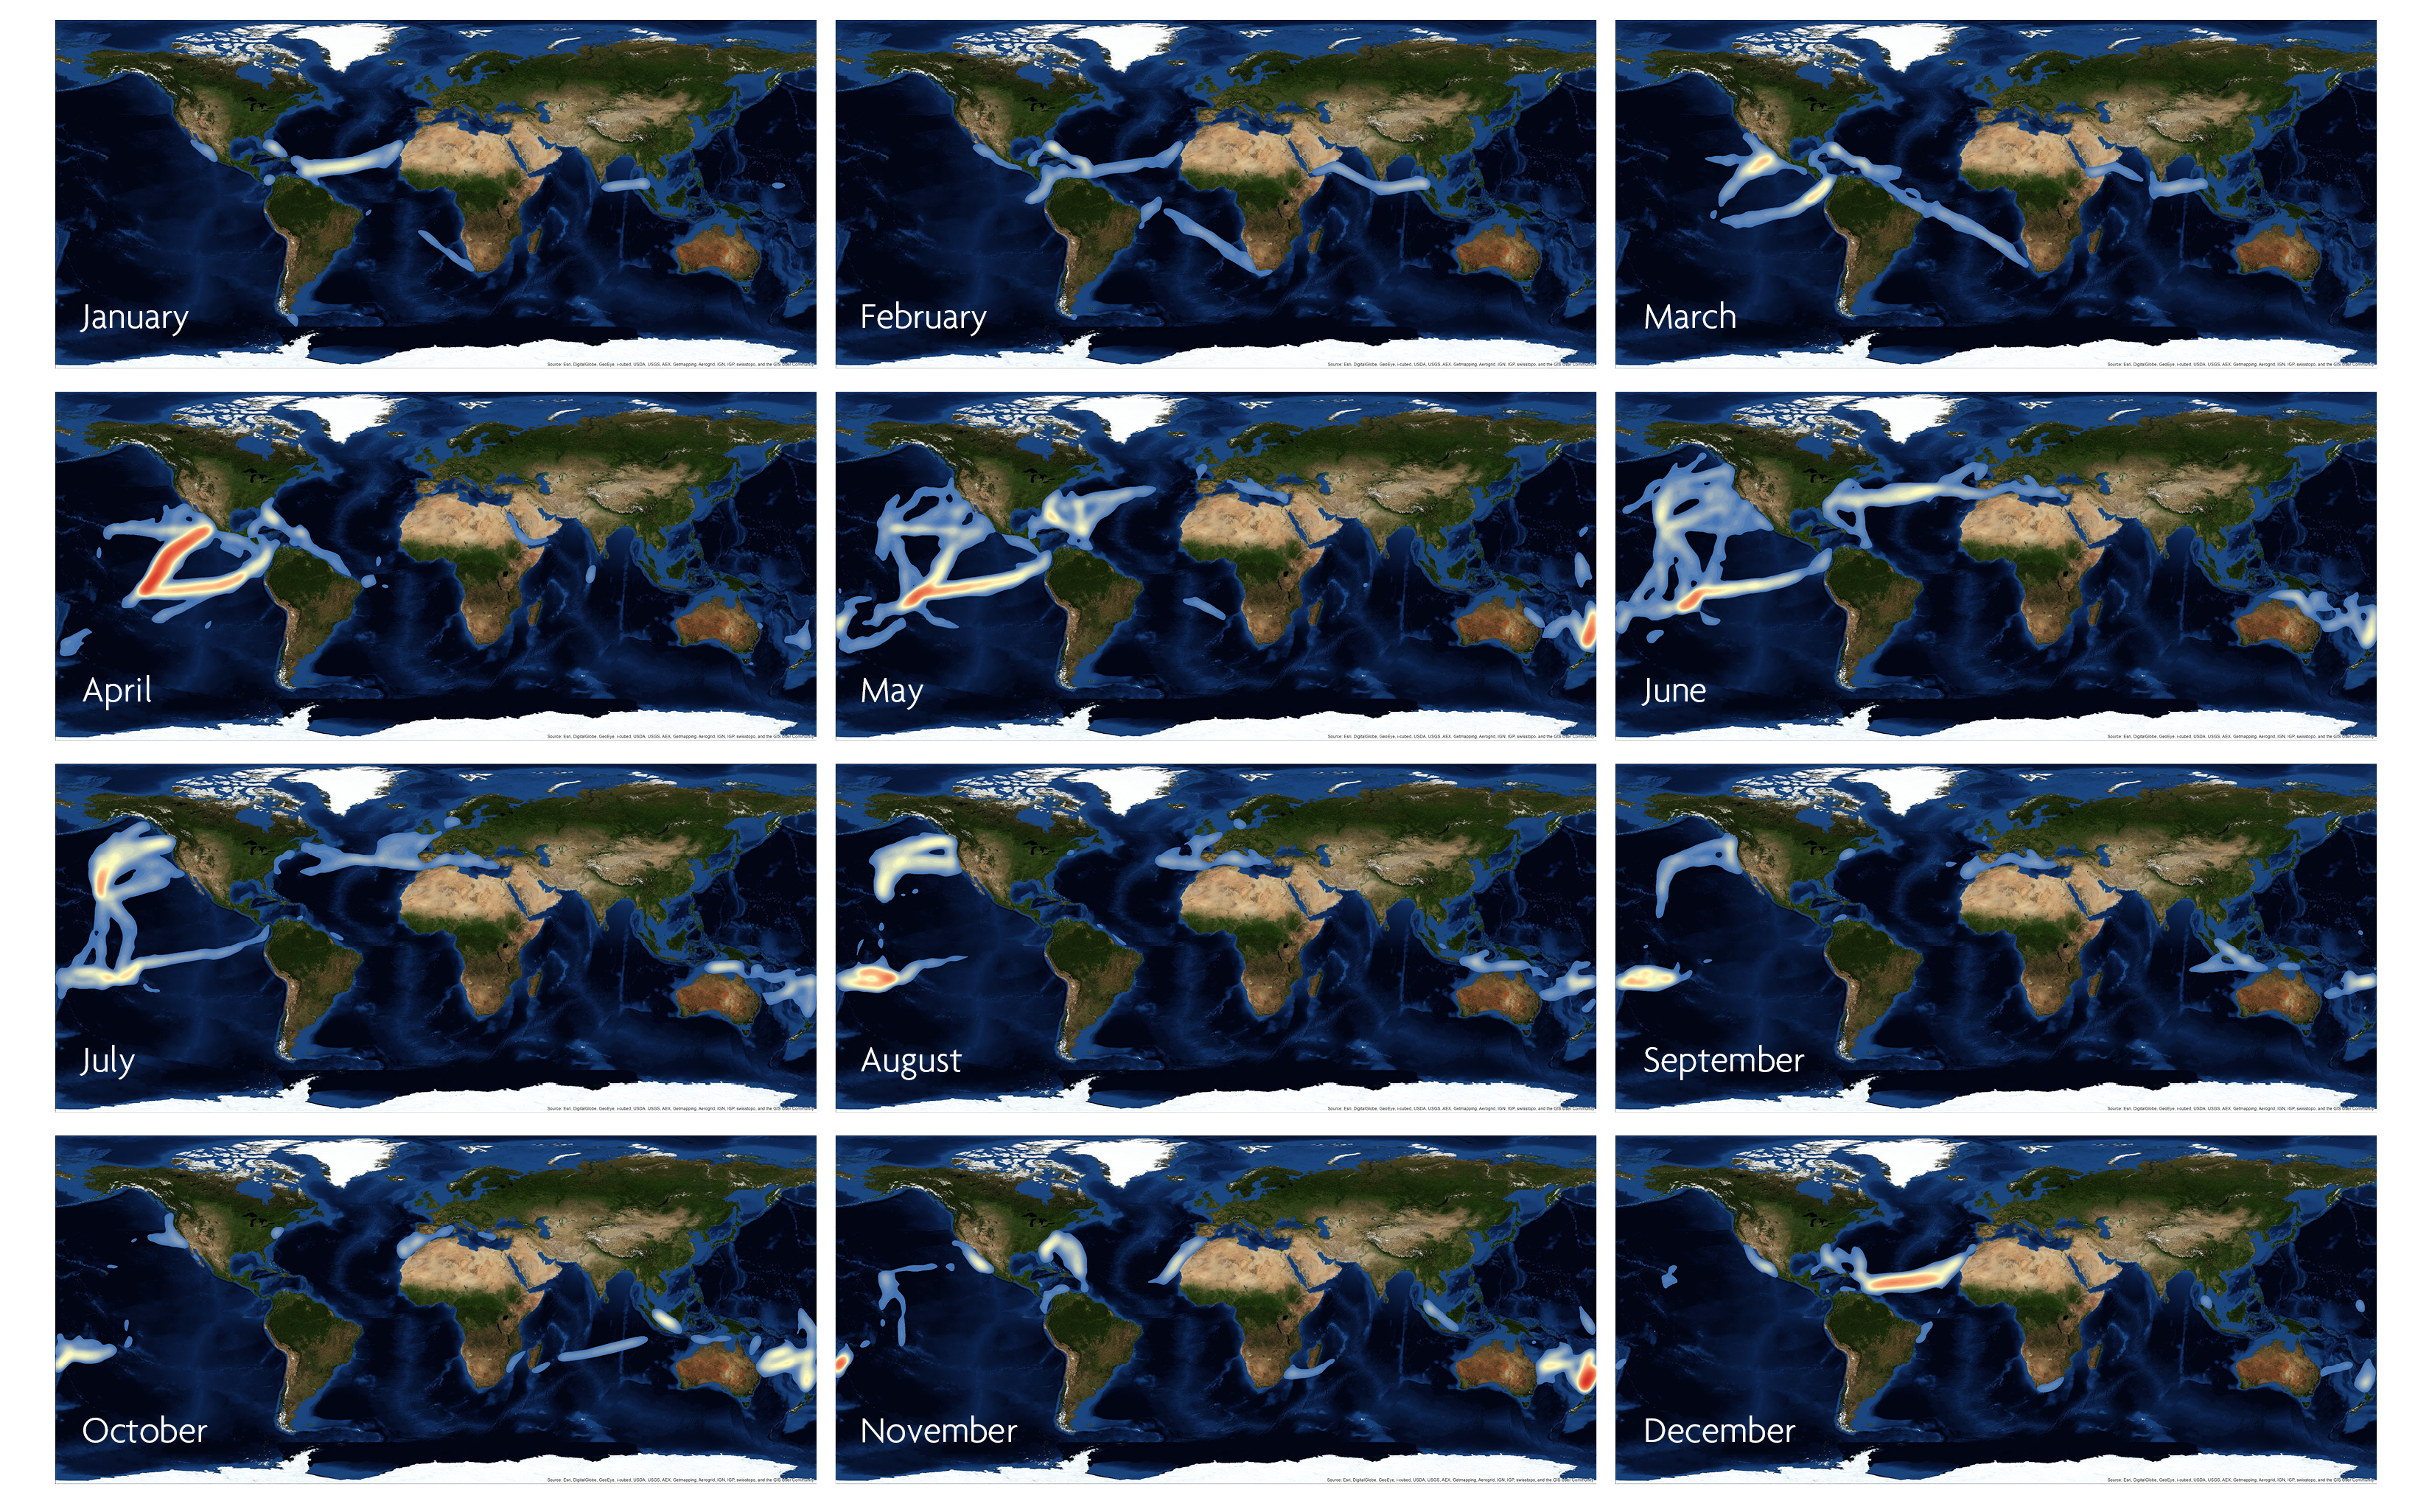
\includegraphics[width=\textwidth]{FishJaws/figures/fig1}
    \caption{\textbf{Pharyngognathy affects dietary transitions in marine fishes.} \textbf{(A)} Four transitions to pharyngognathy on a time-calibrated phylogeny of 851 marine spiny-finned fishes: (1) labroid fishes, including wrasses (Labridae), parrotfish (Scaridae), and weed whitings (Odacidae); (2) surfperches (Embiotocidae); (3) damselfishes (Pomacentridae); (4) marine halfbeaks (Hemirhamphidae). \textbf{(B)} Comparison of the transition rate for nonpharyngognathous and pharyngognathous fishes for fish prey and processing-intensive prey.}
    \label{FJ_fig1}
\end{figure}

To assess the impact of pharyngognathous predators on competition with nonpharyngognathous predators, we investigated feeding performance and functional morphology of cichlids and Nile perch. We measured pharyngeal gape in Nile perch, which possess unfused pharyngeal jaws typical of nonpharyngognathous spiny-finned fishes, as well as in every major lineage of fish-eating cichlid (see Methods). We found that pharyngognathy reduced cichlid pharyngeal gape to half that of Nile perch (Figure \ref{FJ_fig2}A). The only exception to this pattern was in the South American genus Cichla, an old fish-eating cichlid lineage that has independently lost pharyngognathy via loss of fusion of the lower pharyngeal jaw.

\begin{figure}
    \centering
    \includegraphics[width=\textwidth]{FishJaws/figures/fig2}
    \caption{\textbf{Cichlids exhibit reduced pharyngeal gape and increased handling times relative to Nile perch.} \textbf{(A)} Pharyngeal gape comparison of Nile perch, which possesses typical pharyngeal jaws, and fish-eating cichlids, including the one known loss of pharyngognathy in cichlids (genus {\em Cichla}). From top, {\em Lates niloticus}, {\em Harpagochromis} sp. ``orange rock hunter,'' {\em Pyxichromis orthostoma}, {\em Harpagochromis cf serranus}, {\em Harpagochromis} sp. ``two stripe white lip,'' {\em Lipochromis} sp. ``matumbi hunter,'' {\em Lipochromis parvidens}, {\em Champsochromis caeruleus}, {\em Nimbochromis} sp., {\em Rhamphochromis longiceps}, {\em Boulengerochromis microlepis}, {\em Bathybates minor}, {\em Lepidiolamprologus profundicola}, {\em Cyphotilapia frontosa}, {\em Cichla ocellaris}, {\em Parachromis} sp., {\em Petenia splendida}. \textbf{(B)} Handling time comparison between Nile perch and four species of fish-eating Victorian cichlids with respect to the ratio of prey length:predator length. Colors as in (A).}
    \label{FJ_fig2}
\end{figure}

Feeding experiments indicate that pharyngognathy drastically increases handling time in cichlid predators relative to Nile perch. We measured handling time (see Methods) in four predatory Lake Victoria cichlids and similarly-sized Nile perch by using fish prey of sizes and shapes comparable to those consumed in the wild by both groups. \cite{van_oijen_ecological_1982} Cichlids were considerably slower, often taking many hours to process a prey item that a Nile perch could swallow in a few minutes (Figure \ref{FJ_fig2}B). If processing time is examined with respect to pharyngeal gape (see Methods), the difference between Nile perch and cichlids disappears, suggesting that the narrower pharyngeal gape of the cichlids is the primary cause of their long prey-processing times (see Methods). Our results here are limited to predatory cichlids and Lates, but we suggest that similar analyses across marine lineages are likely to be of great interest for understanding the role of pharyngognathy in marine ecosystems.

If pharyngognathy hinders cichlid feeding performance when processing fish prey, fish-eating cichlids may have been particularly disadvantaged after Nile perch were introduced into Lake Victoria. We used conditional inference forests with corrections for correlated variables to explore how ecological variables predict extinction in Victorian cichlids (see Methods). A fish diet is the most important predictor of extinction (Fig. 3A), suggesting that competition played an important role in addition to known factors like predation \cite{witte_destruction_1992} and eutrophication. \cite{seehausen_cichlid_1997, van_rijssel_adaptive_2013}

\begin{figure}
    \centering
    \includegraphics[width=\textwidth]{FishJaws/figures/fig3}
    \caption{\textbf{Extinction of fish-eating Lake Victoria cichlids.} \textbf{(A)} Relative importance of the four highest ecological variables predicting extinction in Victorian cichlids for the original 1992 data set \cite{witte_destruction_1992} and an updated one (see Methods). Pluses indicate increased risk; minuses indicate reduced risk. AUC, area under the curve. \textbf{(B)} Beeswarm plot of size-corrected lower-jaw length of Nile perch (NP), preinvasion Victorian cichlid fish-eaters (LV), postinvasion relict fish eaters (LVrelict), and eight transitions to fish-eating in Lake Tanganyika (LT) cichlids. Large bars indicate mean jaw length.}
    \label{FJ_fig3}
\end{figure}

Of the major functional morphological traits associated with the radiation, a large lower jaw length shows the strongest association with a fish diet in Victorian cichlids. \cite{greenwood1981haplochromine} We reveal a large morphological shift in this character when comparing all fish-eating Victorian cichlids to a representative sample of fish-eaters in the relict fauna of Lake Victoria after Nile perch invasion (Figure \ref{FJ_fig3}B). The preextinction fish-eater community was highly diverse and species rich, with many species possessing jaws of equal or greater size to Nile perch and often consuming large prey. \cite{van_oijen_ecological_1982} However, the few relict fish-eating individuals collected postextinction all have a less predatory morphology than was typical for predatory cichlids of this radiation before the extinction events. The relict Victorian cichlid species now more closely resemble the less-extreme fish-eaters from Lake Tanganyika, where Nile perch and cichlids have coexisted for millions of years. Interspecific competition is thought to be a pervasive force in evolution (29, 30), \cite{pfennig2012evolution, rabosky_diversity-dependence_2013} and we suggest that the pattern we observe across Lakes Victoria and Tanganyika is likely due to competition between Nile perch and cichlid predators.

For nearly half a century, the robust pharyngeal jaws of cichlids, wrasses, and other pharyngognathous fishes have been considered a classic example of evolutionary innovation that opened up new niches through increased trophic flexibility. \cite{liem_evolutionary_1973} Although this is almost certainly correct, our results suggest that the innovation involves a major trade-off that severely limits the size of prey that can be eaten, facilitating competitive inferiority in predatory niches and extinction in the presence of a predatory invader lacking the innovation. The evolutionary innovation of pharyngognathy is not a uniformly beneficial trait, but a specialization that can promote competitive exclusion and extinction depending on ecological context and community composition.
